%\section{Introduction}
Recent studies have shown that advances in machine learning can
improve the prospects for measurements at the Large Hadron Collider~\cite{Baldi:2014kfa,Baldi:2014pta}.
In this paper we explore a machine learning technique, that
has not previously been used inside the high energy physics community: regression with deep neural networks. We apply this method to
the difficult problem of measuring longitudinal Vector Boson Scattering,
which is integral to  electroweak symmetry breaking (EWSB) in the Standard Model (SM).

The discovery of a Higgs-like boson at the
LHC~\cite{ATLAS_higgs,CMS_higgs} was the first step toward a better
understanding of the EWSB mechanism, yet the full picture of EWSB remains to be determined. 
One important, and unverified, prediction of the SM is that the scattering amplitude of longitudinal vector
bosons ($V_{L}V_{L} \rightarrow V_{L}V_{L}$) is unitarized by the
Higgs boson.  Measuring VBS processes at a hadron collider, however,
is experimentally challenging. 
 The ATLAS and CMS collaborations recently provided the first evidence for
 and study of a VBS process using events with two same-electric-charge $W$ bosons in association
with two forward jets ($pp \to$ \ssWW)~\cite{ATLAS_ssWW,CMS_ssWW}.
This final state has the advantage of relatively small SM background
contributions compared to other VBS processes, paired with a
production rate large enough to measure in early LHC data sets.  While
an ideal candidate for first observation of the VBS process, measuring
the longitudinal fraction in these events is not straight forward.

In general, the polarization of a gauge boson can be determined from
the angular distribution of its decay products. The normalized differential cross section of a
leptonically-decaying $W$ boson can be written in terms of
polarization fractions as~\cite{Wpol}:
\begin{multline}
 \label{eq:pol}
 \frac{1}{\sigma} \frac{d\sigma}{d\cts} = \frac{3}{8} f_- (1 \mp \cts)^2 + \frac{3}{8} f_+ (1 \pm \cts)^2 \\ 
+\frac{3}{4} f_L (1 - \ctsSq) , {\text {for~}} W^\pm 
\end{multline}
%  R. Ellis, W. Stirling, and B. Webber, QCD and collider physics
%, Camb. Monogr. Part. Phys. Nucl. Phys. Cosmol. 8 (1996) 1
where \ts is the angle between the charged lepton in the boson
rest frame and the $W$ boson direction of motion.  Fraction
parameters $f_{-}$, $f_{+}$ and $f_L$ denote the fractions of
events with the three possible polarization states of the $W$ boson, $-1$, $+1$ and 0,
respectively.  They are constrained via $f_- + f_+ + f_L = 1$.  In
order to measure \ts, we need to fully reconstruct the direction of
motion of the $W$ boson.

Requiring both $W$ bosons to decay leptonically in  $pp
\to$ \ssWW events enables the determination of the electric charge of
each $W$ boson via the charged leptons. However, since the
corresponding two neutrinos in the final state are not detected, the
$W$ boson rest frames cannot be directly measured.  It is thus
difficult to determine polarization fractions of each boson and
the fraction of longitudinal scattering events in the \ssWW process.

Many proposals have been made to determine the longitudinal fractions in other VBS final states, such as semi-leptonic
$W^+W^-$~\cite{Han:2009em} and $W^\pm Z$~\cite{VBSCuts1} or
fully-leptonic decay modes of $W^\pm Z$ and $ZZ$, where the full
event kinematics can be reconstructed or estimated using the $W$ boson mass constraint. 
However, these channels suffer from large SM backgrounds from gluon initiated processes that result in the same final state. At tree level these processes are not present in the \ssWW channel because of charge conservation. Attempts have been made 
to gain sensitivity through other variables~\cite{VBSCuts1,VBSME,Doroba:2012pd} than \ts in the \ssWW
channel. One example is the variable $R_{pT}=(p_{T}^{\ell 1} \times
p_{T}^{\ell 2}) / (p_T^{j_1} \times p_T^{j_2})$~\cite{Doroba:2012pd},
where $\ell_1$ and $\ell_2$ denote the two leptons in no particular
order and $j_1$ and $j_2$ denote the two most energetic jets in the
event. This single variable does not encompass all of the
sensitivity to longitudinal scattering, and better discrimination can
be achieved by combining the available event information with a
machine learning technique. Therefore, we develop a method to use a
neural network (NN) to map measurable quantities to the true \cts values
that contain the event's polarization information. This
approximation mitigates the limitation of missing kinematic information
in this final state, and makes \ssWW a promising channel for observing
the behavior of longitudinal $W$ boson scattering.
 
%\section{Machine learning model}
While it has become a common practice in high energy physics to use
multi-variate techniques to separate signal from background, to the
authors' knowledge multi-variate regression has not been used to
directly measure underlying physics quantities of interest.
In addition, recent success with deep learning in other areas of
HEP~\cite{Baldi:2014kfa,Baldi:2014pta} suggest that deep learning
is well suited to this problem.

\ssWW events have the signature of two quarks, two same sign leptons, and
two undetected neutrinos.  We use all measurable object kinematics as input variables
to the neural network: the transverse momentum ($p_T$), pseudorapidity ($\eta$) and
azimuthal angle ($\phi$) of the two leptons and two jets, and $x$- and $y$-components 
of missing transverse energy ($\slashed{E}_T^x$ and
$\slashed{E}_T^y$).  The overall number of measurable quantities used hence is 14. 
The goal of the multi-variate technique is to find
the best mapping from these measurable quantities to the two truth
values of \cts (one for each $W$ boson) present in each event.  We
choose a multi-layer neural network with a final output layer \fixme{mention two nodes output already here?!} with
linear activation. The neural network is implemented with the Theano
software packages~\cite{theano1,theano2}. The cost function is defined as
\begin{equation}
 \label{eq:cost}
{\cal{C}}= \frac{1}{N}\sum_{i=1}^{N} [(\ctsnb_{1,i} -\cos \theta^{NN}_{1,i})^2+(\ctsnb_{2,i}-\cos \theta^{NN}_{2,i})^2],
\end{equation}
where $N$ is the number of events per mini-batch,
$\ctsnb_{1/2,i}$ is the truth value of \cts for each $W$ boson with
random ordering for the $i$-th event, and $\cos \theta^{NN}_{1/2, i}$ is the value of
the two neural network outputs. A Stochastic gradient descent
algorithm is used to train the neural network. Hyper-parameters are tuned by hand and confirmed
by a local grid search, with the best performance given by a deep network with 20 layers each with 200 hidden nodes.
This network yields a 20\% better cost value in a validation data set than the best single layer network tested.   

Signal \ssWW events are generated using the {\sc madgraph} event generator~\cite{madgraph} at a proton-proton center-of-mass energy of 13 TeV. %The NN23l01 {\bf find more correct name for this PDF set} parton distribution function~\cite{pdf} is used as the default. 
 The invariant mass of the two outgoing partons were required to be greater than 150 GeV. The $W$ bosons are decayed, assuming they are on-shell and have no spin correlations, with the {\sc decay} routine provided with {\sc madgraph}.% Events are split into three categories: 1/4 are used in a training sample, 1/4 are used for a validation test against over-training, and the
 %remaining 1/2 are used to build templates and perform sensitivity
%studies.% A ** layer neural network with ** hidden neurons and a
%learning rate of ** is used {\bf I can move thie earlier, but I also didn't use a fixed learning rate }.

%\section{\label{sec:signal} Signal Model}
Polarization fractions can then be obtained experimentally by fitting the two-dimensional distribution of the NN output \ctsNN.  
In order to fit for these polarization fractions templates must be built for ``pure'' polarization states. These
templates are created using generator level helicity information. In addition, a method was tested that used truth level reweighting and included all spin correlations and off-shell effects, the results were comparable.

%% by reweighting each event based on the truth
%% \cts distribution. The event weight $W_i$ for polarization state $i$ is given by
%% $W_i = F_i/n$, where $n$ is used for the normalization and is
%% defined as
%% \begin{multline}
%% n=[ \frac{3}{8} f_- (1 \mp \ctsnb_1)^2 + \frac{3}{8} f_+ (1 \pm \ctsnb_1)^ 2 +\frac{3}{4} f_L (1 - \ctsSqnb_1)] \\
%% \times [ \frac{3}{8} f_- (1 \mp \ctsnb_2)^2 + \frac{3}{8} f_+ (1 \pm \ctsnb_2)^ 2 +\frac{3}{4} f_L (1 - \ctsSqnb_2)]. 
%% \end{multline}
%% The index $i$ represents one of six possible polarization states for the two
%% $W$ bosons: Left-Left ($--$), Left-Right ($-+$), Right-Right($++$),
%% Left-Longitudinal ($-L$), Right-Longitudinal ($+L$), or
%% Longitudinal-Longitudinal ($LL$) {\bf no reason to name them Left/Right if we are using +/-}. $F_i$ is defined as \small
%% \begin{equation}
%% F_i \in  \left( \begin{array}{c} 
%%   --=f_-^2 (1 \mp \ctsnb_1)^2(1 \mp \ctsnb_2)^2,\\
%%   -+=f_- f_+[ (1 \mp \ctsnb_1)^2(1 \pm \ctsnb_2)^2\\ \;\;+(1 \pm \ctsnb_1)^2 (1 \mp \ctsnb_2)^2],\\
%%   ++=f_+^2 (1 \pm \ctsnb_1)^2(1 \pm \ctsnb_2)^2,\\
%%   -L=f_- f_L[ (1 \mp \ctsnb_1)^2(1 - \ctsSqnb_2)\\  \;\;+(1 - \ctsSqnb_1))(1 \mp \ctsnb_2)^2 ],\\
%%   +L=f_+ f_L[ (1 \pm \ctsnb_1)^2 (1 - \ctsSqnb_2))\\  \;\;+(1 - \ctsSqnb_1)(1 \pm \ctsnb_2)^2 ],\\
%%   LL=f_L^2 (1 - \ctsSqnb_1))(1 - \ctsSqnb_2)\\
%% \end{array} \right).
%% \end{equation}
%% \normalsize Since no ordering is applied to the two bosons we require
%% that the individual polarization fractions $f_-$,$f_+$,$f_L$ are the
%% same for both $W$ bosons.  For reweighting, the original sample $f_-$,
%% $f_+$, $f_L$ are taken as a function of the invariant mass of the
%% diboson system ($M_{WW}$).  Weights are calculated before any
%% additional event level cuts are made, and the resulting templates are
%% remade for each set of cuts explored.  
%% %To validate the reweighting procedure, we also generate pure polarization state samples using {\sc
%% %  madspin} and compare the obtained events kinematics with those
%% %obtained from the reweighted sample. 
%% {\bf Does this mean you got the
%%   MG5 scripts to work and add the helicity to the lhe? A. No this was never done removed this.}
Since there are two $W$ bosons in each event, six distinct polarization states are possible. Events where both $W$ bosons have a polarization of 0 are referred to as $LL$, of 1 as $++$, and of $-1$ as $--$. Events with differing polarizations of ($-1$,1) or (1,$-1$) are referred to as $+-$, ($-1$,0) or (0,$-1$) as $L-$ and likewise (1,0) or (0,1) as $L+$. 

Fig.~\ref{fig:polarization_comparison}(a) shows the comparison between the truth \cts and 
the NN output \ctsNN for $--$, $++$ and $LL$ events ( $+-/L+/L-$ are omitted for clarity, but closely resemble combinations of the templates shown). As expected, \ctsNN has less separation 
power for the different polarization states compared to \cts due to missing information for the two final state neutrinos. 
However, reasonable discrimination between each polarization state can clearly be seen from these distributions. 
Fig.~\ref{fig:polarization_comparison}(b) shows the $R_{pT}$ distribution for $--$, $++$, and $LL$ events. 
The discrimination power is seen only for large values of $R_{pT}$, and only apparent with a logarithmic scale.

Fig.~\ref{fig:polarization_comparison}(c) shows the \ctsNN
distribution for the signal \ssWW process and the dominant background
process: $WZjj$ production.  Reasonable separation power is observed. In an actual
data analysis, the $WZjj$ component would be subtracted as background
from the observed data before fitting the polarization fractions.

\begin{figure*}
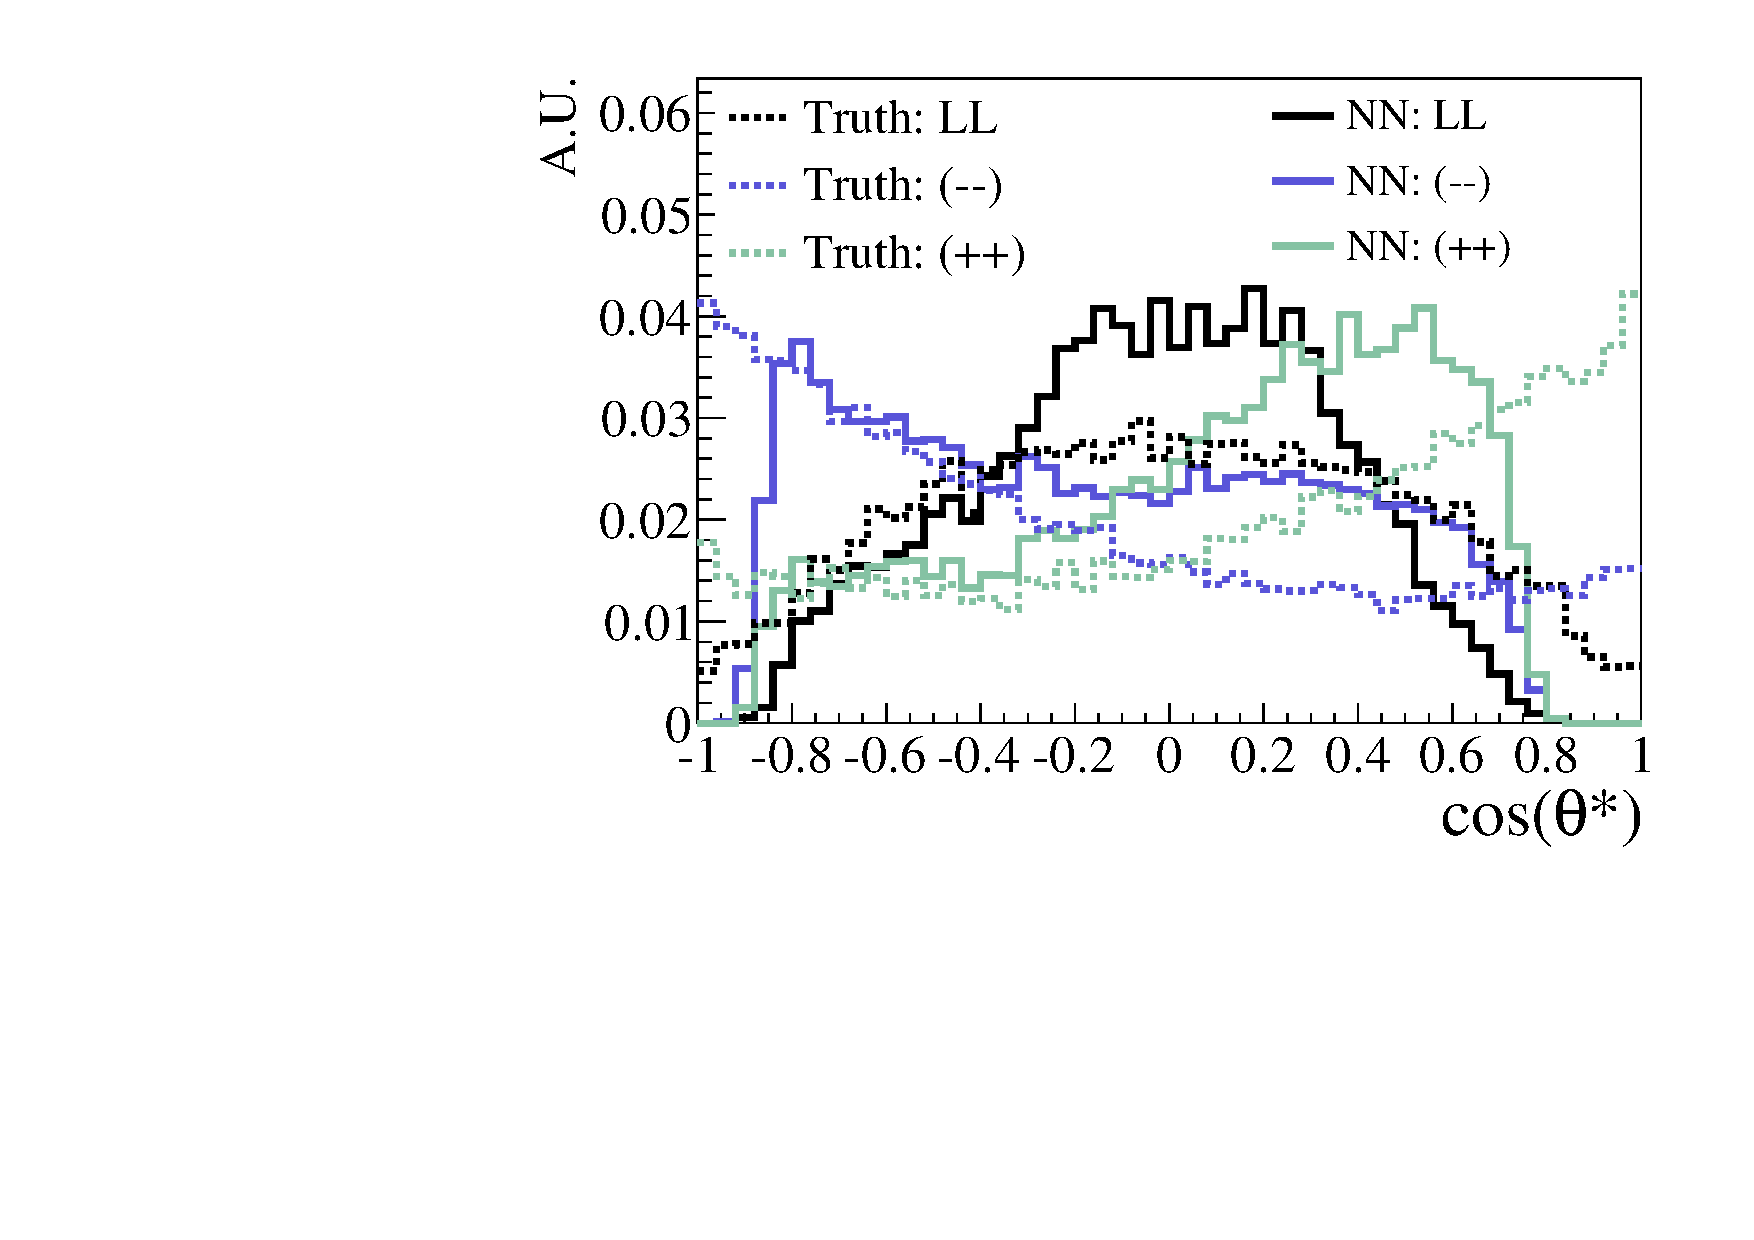
\includegraphics[width=.32\textwidth,height=.18\textheight]{./fig/1d_templates_graph_X.pdf}
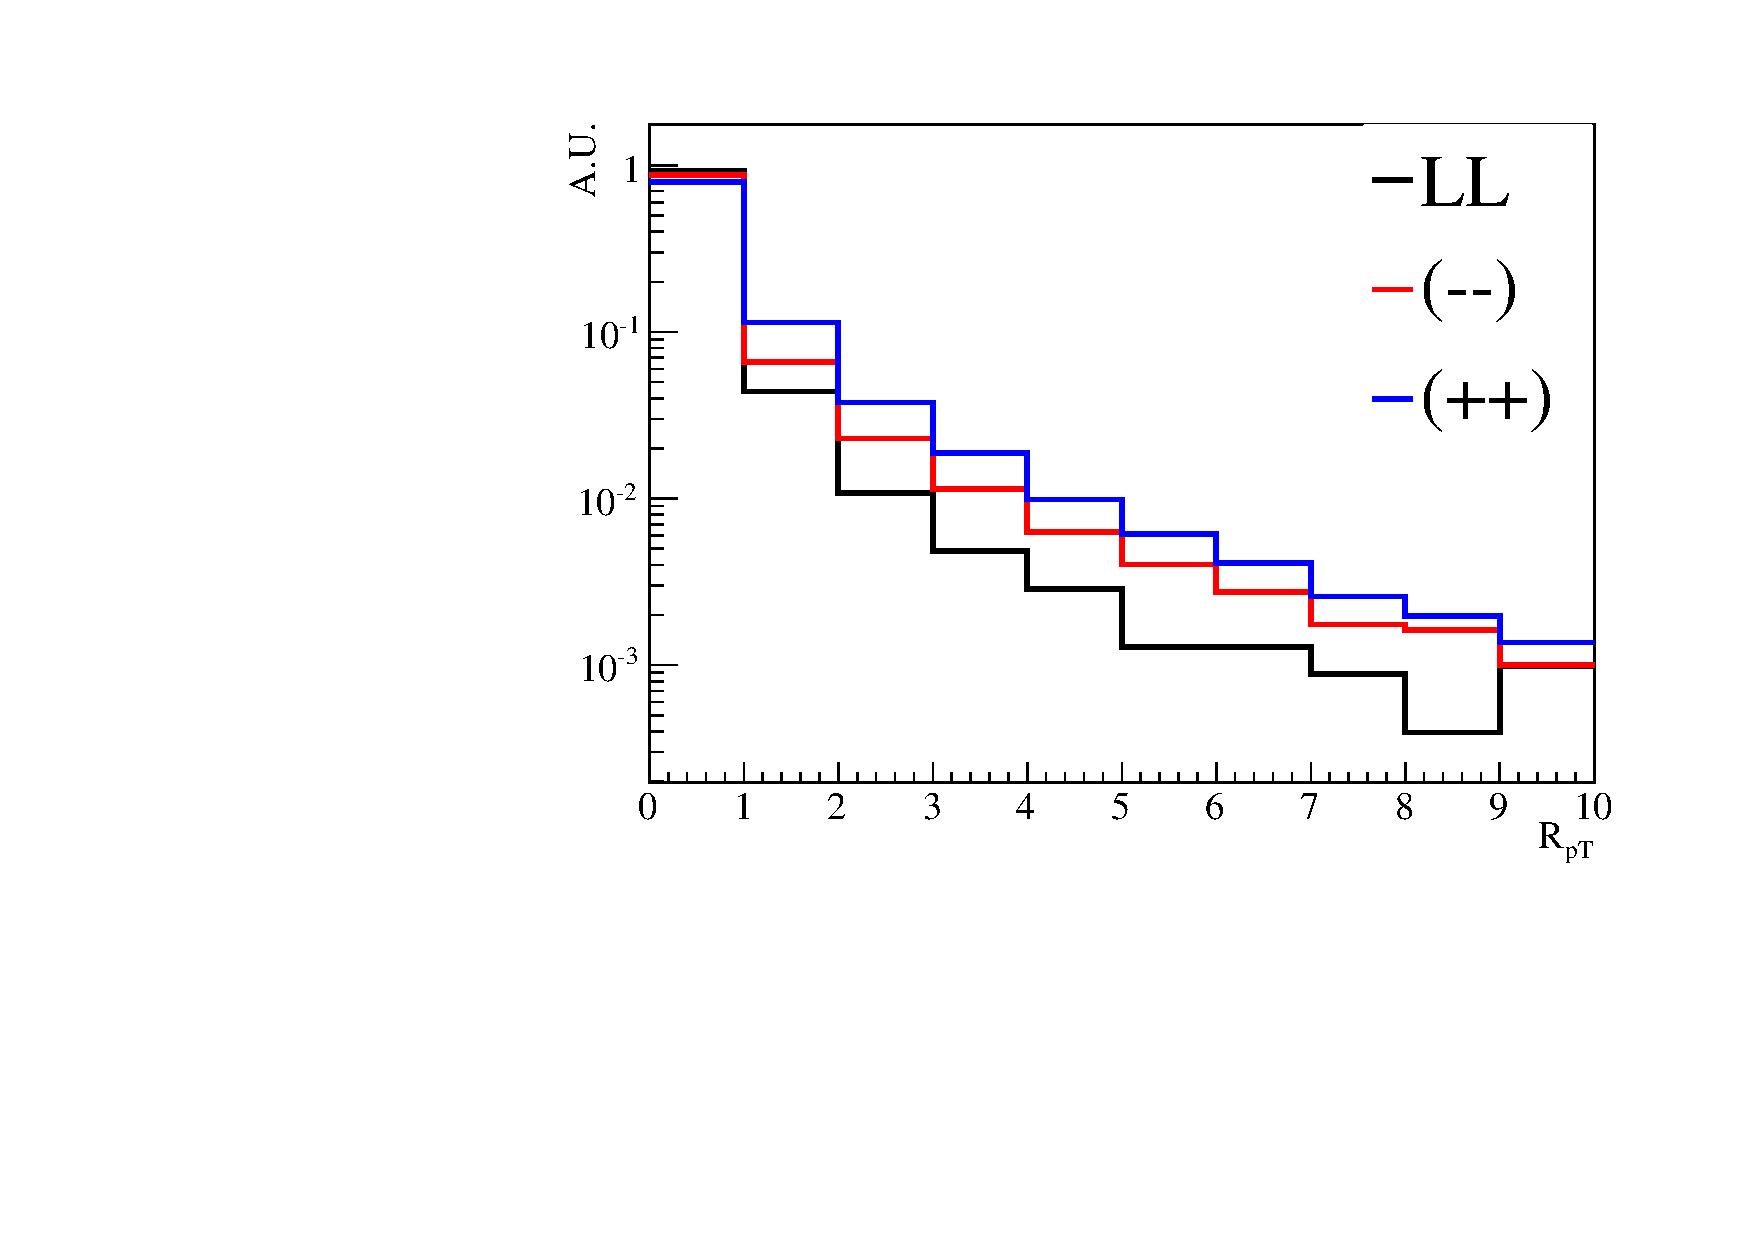
\includegraphics[width=.32\textwidth,height=.18\textheight]{./fig/ratios_LLRROO_graph.pdf}
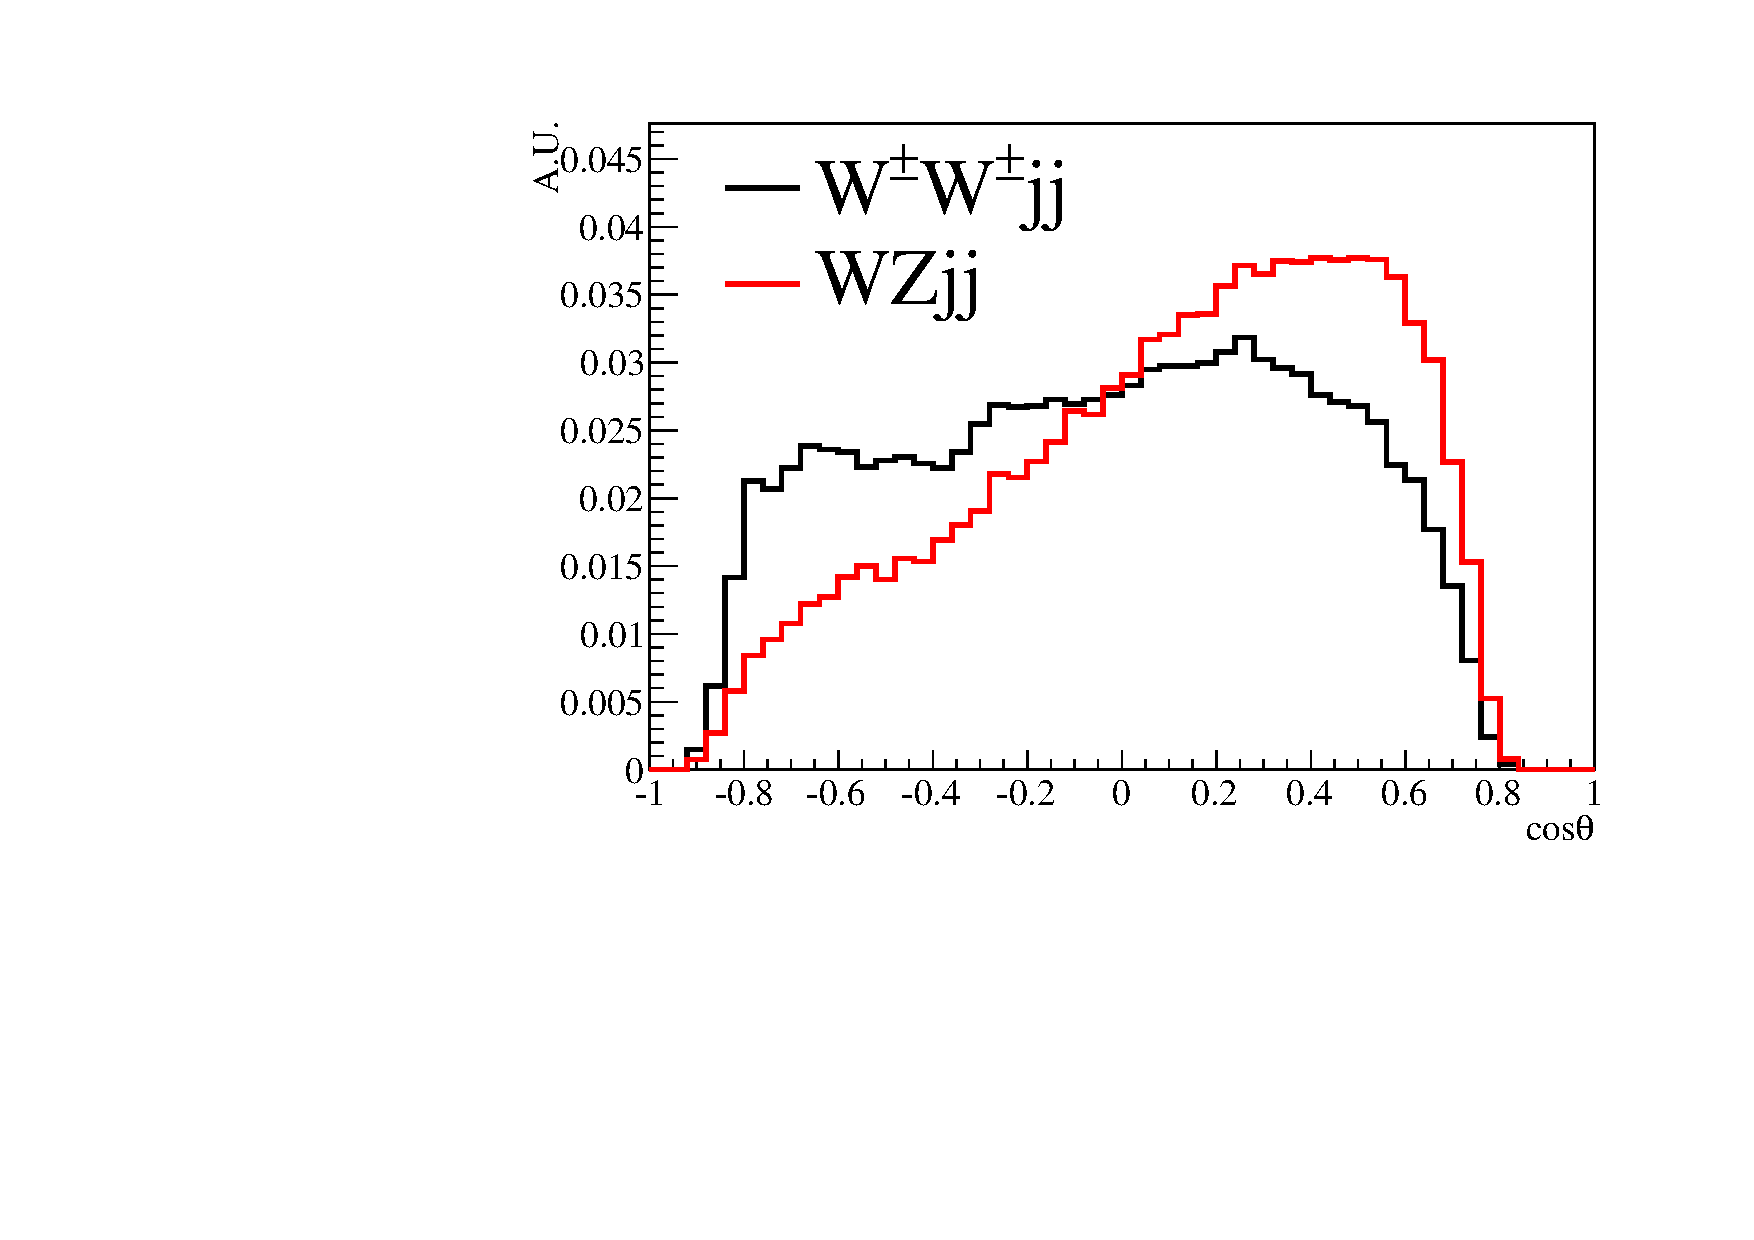
\includegraphics[width=.32\textwidth,height=.18\textheight]{./fig/1d_wz_bg_graph_X.pdf}
\caption{\label{fig:polarization_comparison} Comparison of the truth level \cts and the 
NN output \ctsNN distributions for $--$, $++$ and $LL$ events (Left), 
$R_{pT}$ templates for the corresponding polarization states (Middle), 
and comparison of the \ctsNN for the signal and dominant $WZjj$ background (Right).}
\end{figure*}

%\section{Results}
Having established templates for each polarization state and a
distribution that is sensitive to different polarization states, 
we fit the two-dimensional $\ctsNN_1$ vs. $\ctsNN_2$
distribution in pseudo data to derive each polarization fraction. Five equal-size bins 
are used for each \ctsNN variable ranging from $-1$ to 1. A maximum likelihood fit is performed 
within the RooFit framework~\cite{RooFit}. We combine events with both $W$ bosons transversely-polarized as
``$TT$'' (the sum of $--$, $+-$ and $++$ combinations), events with
one $W$ boson transversely-polarized and one $W$ boson
longitudinally-polarized as ``$TL$'' (the sum of $L-$ and $L+$
combinations), and events with both $W$ bosons
longitudinally-polarized as ``$LL$''. This reduces the free fitting parameters from 5 to 2 and 
allows for a better constraint on the $LL$ scattering fraction of interest, under the assumption that
the relative admixture of contributions within $TT$ and $TL$ does not change. Statistical fit uncertainties are determined by randomly
fluctuating data expectations within their Poisson uncertainties and
repeating the fit, and confidence intervals are derived from these toy experiments.  
%{\bf (need to put more description here about 68\% and 95\% level limits)}
%To validate the fitting method, we also make sure the
%fitted values for each fraction agree with with the values obtained at
%the truth level. {\bf transition from truth level templates to reco
%  level dists not clear; where has NN been used?}

%There are six possible polarization states for the two colliding $W$ bosons. 

Fits are performed in a range of integrated luminosities from $0.01-3$~ab$^{-1}$. An example fit for 1 ab$^{-1}$ is shown in Fig.~\ref{fig:fit_example} where the pseudo data are compared to the sum of 
contributions from $TT$, $TL$ and $LL$ components. It is found that the $LL$ fraction can be measured with a 68\% confidence limit of (6.7$\pm 1.4)\%$ with an ultimate luminosity of 3 ab$^{-1}$. When a similar fit is applied to the $R_{pT}$ variable the precision of (6.7$^{+7.1}_{- 6.7})\%$ is found to be consistent with 0. The regression technique hence greatly enhances the sensitivity to this process.

\begin{figure}[h]
%\begin{overpic}[width=0.49\textwidth,grid,tics=10]{./fig/NN_fit_3.pdf}
\begin{overpic}[width=0.49\textwidth]{./fig/NN_fit_3.pdf}
%% \put (77,-1) {$\ctsNN_1$}
%% \put (7,2.5){\footnotesize$-1$}
%% \put (25,2.5){\footnotesize$1$}
%% \put (22.3,0){\color{red}\footnotesize$-1$}
%% \put (41.3,0){\color{red}\footnotesize$1$}
%% \put (38.7,2.5){\footnotesize$-1$}
%% \put (57.3,2.5){\footnotesize$1$}
%% \put (54.6,0){\color{red}\footnotesize$-1$}
%% \put (73.4,0){\color{red}\footnotesize$1$}
%% \put (70.6,2.5){\footnotesize$-1$}
%% \put (89.3,2.5){\footnotesize$1$}
\put (77,-1) {$\ctsNN_1$}
\put (7,2.5){\footnotesize$-1$}
\put (22.3,2.5){\footnotesize$\pm 1$}
\put (38.7,2.5){\footnotesize$\mp 1$}
\put (54.6,2.5){\footnotesize$\pm1$}
\put (70.6,2.5){\footnotesize$\mp1$}
\put (89.3,2.5){\footnotesize$1$}
\put (77,54) {$\ctsNN_2$}
\put (7,51){\footnotesize$-1$}
\put (21.5,51){\footnotesize$-0.6$}
\put (37.5,51){\footnotesize$-0.2$}
\put (55.5,51){\footnotesize$0.2$}
\put (72,51){\footnotesize$0.6$}
\put (89.3,51){\footnotesize$1$}

\end{overpic}
%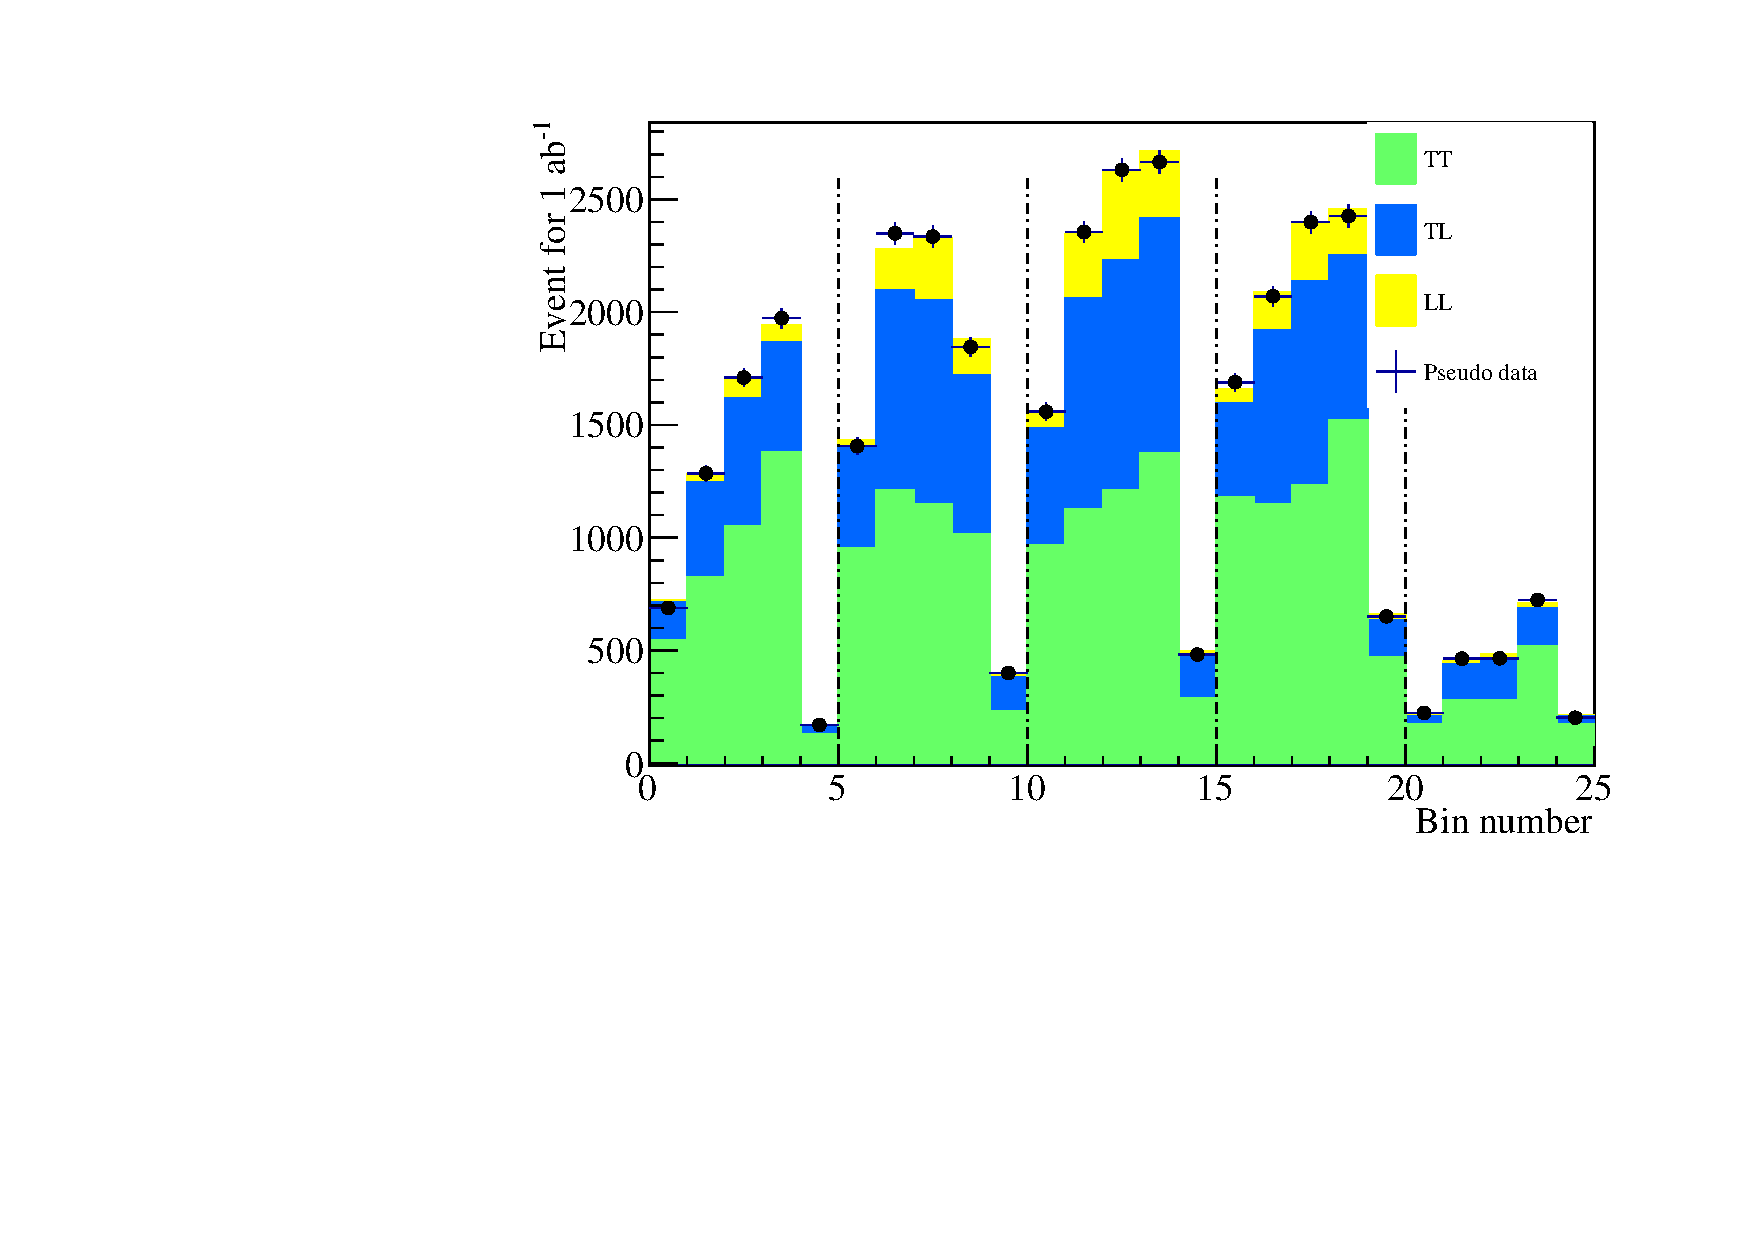
\includegraphics[width=.49\textwidth]{./fig/NN_fit_3.pdf}
\caption{\label{fig:fit_example} One example fit where the pseudo data are compared to the sum of 
contributions from $TT$, $TL$ and $LL$ components. There are five groups with five bins inside each group. 
These five groups represent $\ctsNN_2$ from $-1$ to 1 with a step size of 0.4, while five bins inside each group represent $\ctsNN_1$ from $-1$ to 1 with a step size of 0.4. \fixme{y-axis: ``Event'' $\to$ ``Events''}}
\end{figure}

The above measurements are performed with parton level predictions. While they show encouraging results  it is important 
to also check if this procedure will stand up to experimental reality of finite detector resolution, and the event level selection that
will be required to remove backgrounds from this analysis. To study the effects of event level cuts, we apply additional selection criteria as used by the ATLAS collaboration~\cite{ATLAS_ssWW} to obtain a
tighter fiducial region which is dominated by the contribution from electroweak production of \ssWW events: jet $p_T > 30$ GeV, lepton $p_T > 25$ GeV, missing transverse energy $\slashed{E}_T > 40$ GeV, 
dijet mass $M_{jj} > $500 GeV, and dijet pseudorapidity difference $|\Delta \eta_{jj}| > 2.4 $. 
%If these criteria are applied at the generator level, jet $p_T$, $M_{jj}$ and $\Delta \eta_{jj}$ are calculated using the parton-level jets 
%and $\slashed{E}_T$ are calculated using two generator-level neutrinos.

To emulate the response of a typical general-purpose LHC detector, these events are parton-showered using {\sc pythia}\cite{pythia} and passed through the  response simulation of the CMS detector implemented in {\sc delphes}~\cite{delphes}. Parton level quantities are then approximated by taking the leading two jets clustered with an anti-$k_t$ algorithm~\cite{antikt} with jet size parameter R=0.5.

Backgrounds to the \ssWW process depend largely on experimental choice, and require detailed simulation. It can be seen in Fig.~\ref{fig:polarization_comparison} that background from the $WZjj$ process (where one of 
the leptons from the $Z$ boson decay is not detected) has a different \ctsNN shape than \ssWW events, but it is likely event level cuts will still need to be applied to reduce this component. Determining the systematics on the background shapes will require significant work from the experiments, and is not treated here. However, as already mentioned the backgrounds in the \ssWW channel are relatively small compared to other channels.

\fixme{Boil down to a,b,d scenarios, ordered wrt. increasingly realistic modelling?}
We determine the precision that can be achieved for fractions of $TT$, $TL$, and $LL$ components using four different scenarios: (a) using all  generated events at the parton level; 
(b) using events passing the additional selection criteria used by ATLAS at the parton level; 
(c) using all generated events processed with the {\sc delphes} detector simulation; and (d) using events processed with the {\sc delphes} detector simulation and with reconstructed objects passing additional selection criteria used by \mbox{ATLAS}. 

\begin{figure*}
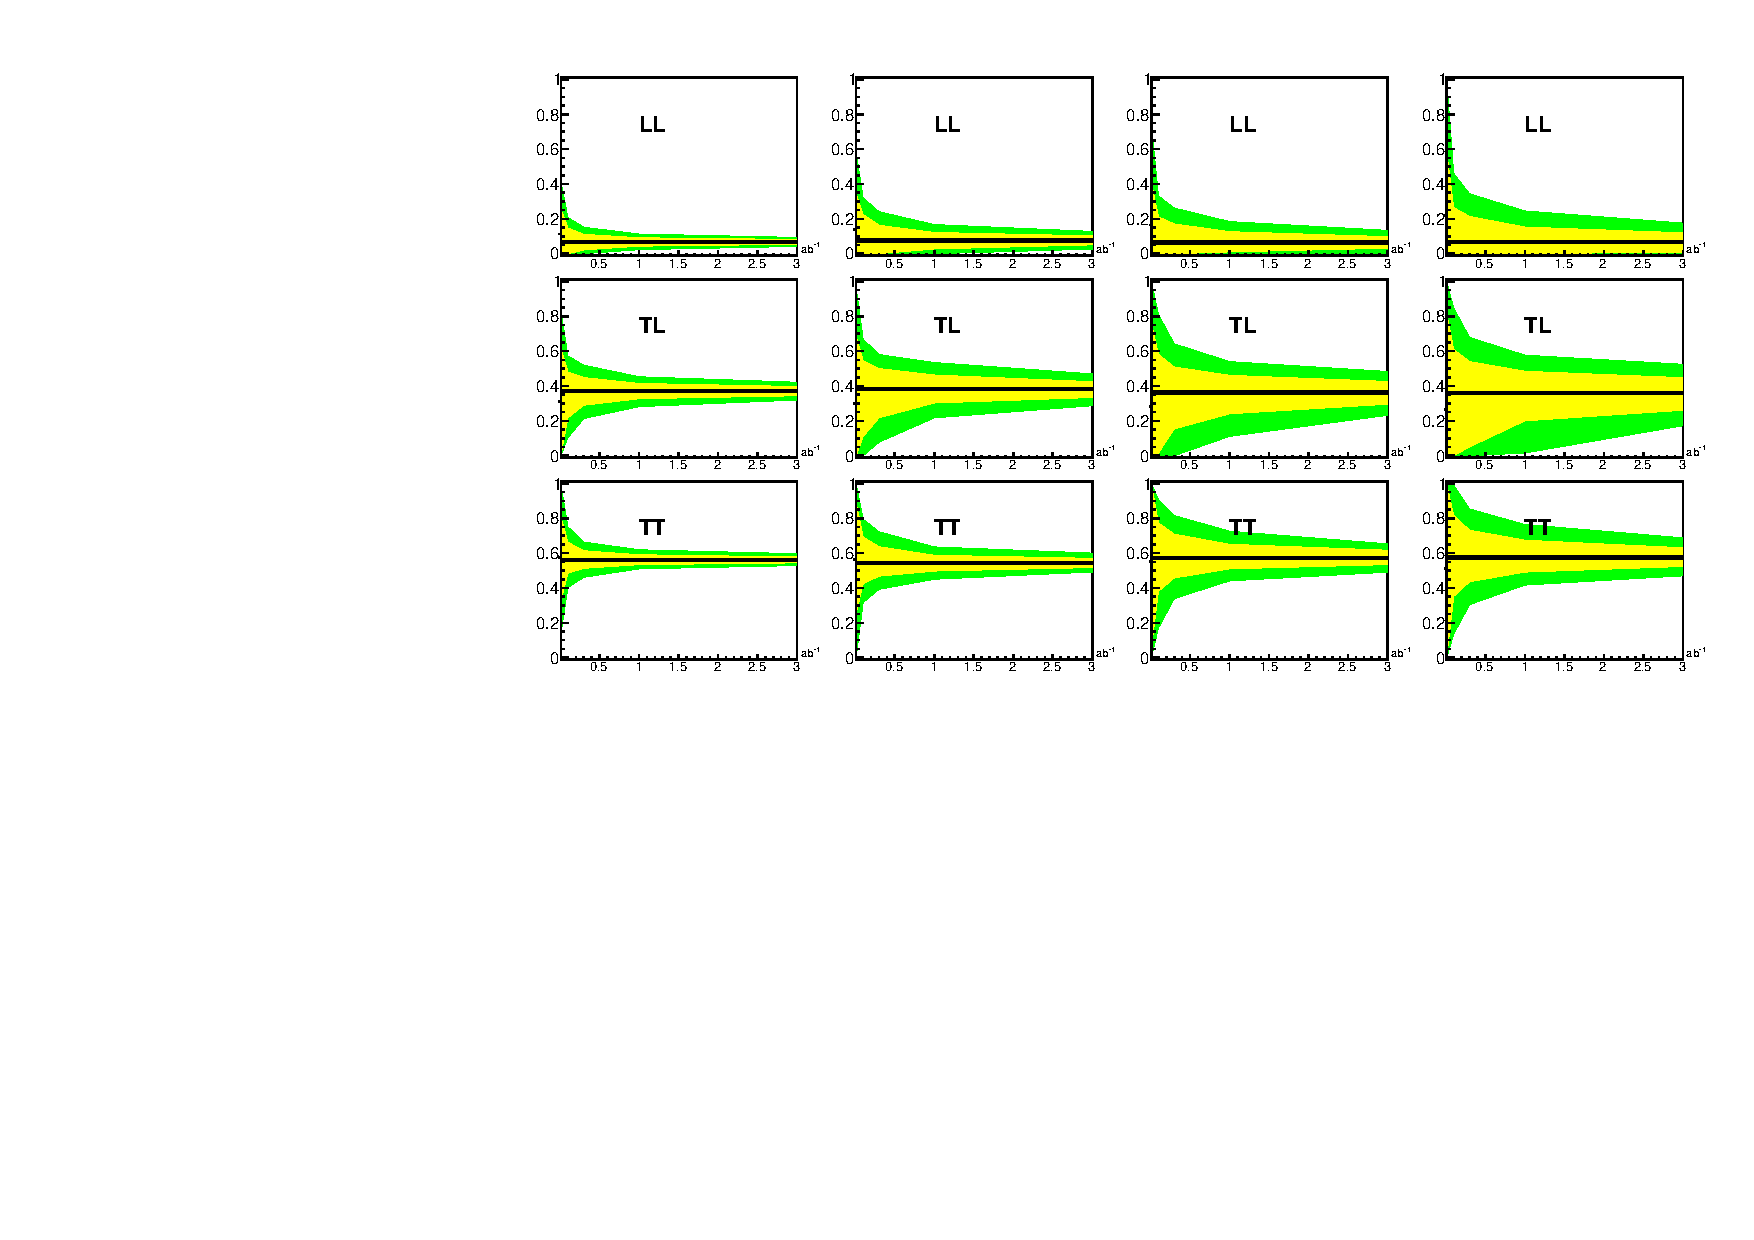
\includegraphics[width=.9\textwidth]{./fig/12_LL_LT_TT.pdf}
\caption{ \label{fig:sensitivity} 68\% (yellow) and 95\% (green) confidence intervals for the LL (top), TL (middle), and TT (bottom) polarization fractions as a function of the integrated luminosity for from left to right scenarios (a),(b),(c), and (d) discussed in the text. \fixme{Add proper x/y axis labels, e.g. $f_{TT}$ etc. on y-axis?}}
\end{figure*}

The precision for the three polarization fractions as a function of the integrated luminosity is presented in Fig.~\ref{fig:sensitivity}. 
 TT components can be measured with great precision, whereas separating pure LL scattering from LT scattering is challenging.
In the most difficult scenario (d), the cuts slightly increase the mean $LL$ fraction to 7.0\% and 68\% confidence limits are found 7$^{+19}_{-7}$\% (7$^{+5}_{-6}\%$) for an integrated luminosity of 0.1 (3) ab$^{-1}$.  Equivalent limits from fits to $R_{pT}$ variable are found to be 7$^{+29}_{-7}\%$ and 7$^{+9}_{-7}\%$. The fit to the neural network almost doubles the ultimate precision to anomalous $LL$ fractions in this scenario. Reaching the same statistcal senstivity using the $R_{pT}$ variable would require approximatly 10 ab$^{-1}$, more than 3 times the total LHC program. We have shown that large sensitivity gains can be made with Neural Network regression. In scenario (d) our simple estimate falls short of the $5\sigma$ criteria for observation of longitudinal VBS, however, stringent limits on new physics can be set. In addition, the authors hope that experiments can improve on this methodology by training on fully simulated events or by improving detector performance through upgrades to enhance sensitivity and eventually complete the EWSB picture. 
\fixme{Add stronger statement along the lines: ``if SM is wrong, LL could be dramatically enhanced~\cite{VLVLBSM}, so an improved capability to set limits on $f_{LL}$ will be key to use VBS as a window to new physics phenomena.'' Might also need to mention this already in the introduction?}

%\section{Conclusions}
In conclusion, we present a method to determine the $WW$ polarization fractions in
\ssWW events by using a deep machine learning technique.  This method
allows to recover the charged lepton angular distributions in the $W$
boson rest frame from measurable event kinematics.  The
results obtained from this method show greatly enhanced sensitivity over
the example $R_{pT}$ variable.  Cuts to reject
backgrounds as well as finite detector resolutions reduces the sensitivity as
expected, but the method remains a powerful tool for the study of
polarization fractions in VBS events, almost doubling the ultimate precision when compared to a previously explored sensitive variable.

We would like to thank our colleagues Sally Dawson and Olivier Mattelaer for their help and guidance while preparing this manuscript.
The contributions from JS, LH and JZ were supported by the Department of Energy Early Career Grant under contract DE-SC0008062. The work of M-AP is supported by DOE Contract No. DE-SC0012704. \fixme{ATLAS scholarship to be added for JS}

\bibliographystyle{myutphys}
\bibliography{ref}

